\begin{surferIntroPage}{Singularidades simples}{simplesing_A1pm}{Singularidades simples}
Se dice que una superficie es \emph{lisa} o \emph{no singular}
si, en términos intuitivos, no tiene puntas, pliegues o aristas
(estos puntos especiales se dice que son \emph{singulares}).
Las dos primeras imágenes abajo, la esfera y el toro,
son ejemplos de superficies lisas:
    \begin{center}
      \vspace{-0.2cm}
      \begin{tabular}{@{}c@{}c@{}c@{\quad}c@{}c@{}c@{}c@{}}
        \begin{tabular}{@{}c@{}}
          Lisas:
        \end{tabular}
        &
        \begin{tabular}{@{}c@{}}
          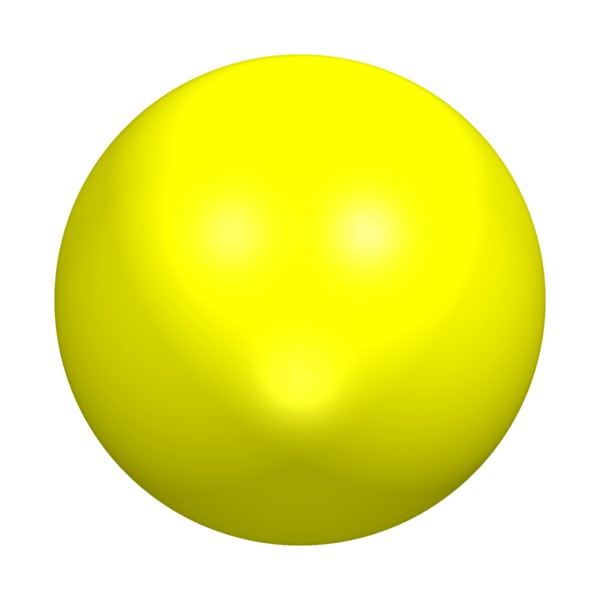
\includegraphics[width=1.1cm]{../../common/images/kugel}
        \end{tabular}
        &
        \begin{tabular}{@{}c@{}}
          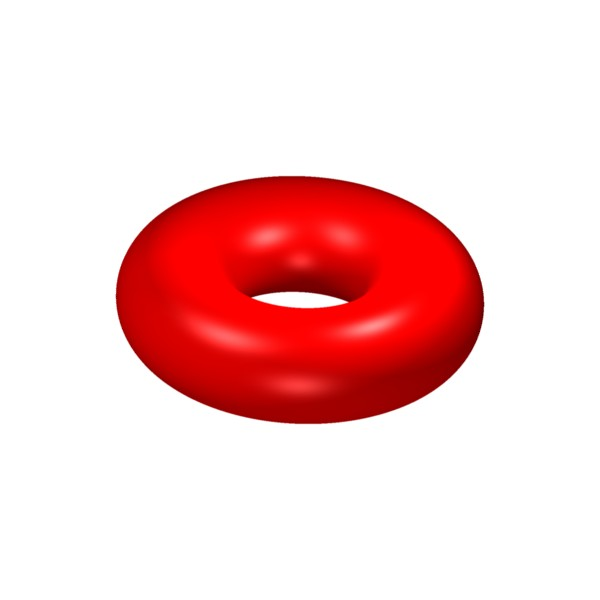
\includegraphics[width=1.1cm]{../../common/images/torus}
        \end{tabular}
        &
        \begin{tabular}{@{}c@{}}
          Singulares:
        \end{tabular}
        &
        \begin{tabular}{c@{}@{}}
          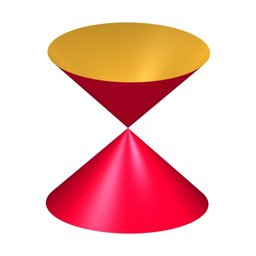
\includegraphics[width=1.1cm]{../../common/images/kegel}
        \end{tabular}
        &
        \begin{tabular}{c@{}@{}}
          \includegraphics[width=1.1cm]{../../common/images/A2pm}
        \end{tabular}
        &
        \begin{tabular}{c@{}@{}}
          \includegraphics[width=1.1cm]{../../common/images/A3pm_0}
        \end{tabular}
      \end{tabular}
    \end{center}
    \vspace{-0.2cm}
Las singularidades más simples son conocidas como \emph{ADE}, como
por ejemplo las de tipo
$A_k^{\pm\pm}$, definido por la ecuación
    $x^{k+1}\pm y^2\pm z^2=0$.
La superficie azul en la imagen tiene un punto singular de tipo
$A_3^{+-}$, la de color magenta, de tipo
$A_2^{+-}$, y la de color rojo (llamada \emph{cono cuadrático}),
de tipo $A_1^{+-}$.
Las singularidades ADE tienen sorprendentes relaciones, aún no bien
entendidas, con numerosas ramas de las matemáticas y la física, y con
la naturaleza. Cada $A_k$
se puede deformar en $\lfloor\frac{k+1}{2}\rfloor$
singularidades $A_1$; de una
$A_3^{+-}$, se obtienen dos $A_1^{+-}$ (imágenes abajo a la
izquierda):
%\vspace*{-3pt}
%    \dontshow{
    %
    \begin{center}
      \vspace{-0.2cm}
      \begin{tabular}{@{}c@{\quad}c@{}c@{\qquad\quad}c@{\quad}c@{\quad}c@{}}
        \begin{tabular}{@{}c@{}}
          \includegraphics[width=1.2cm]{../../common/images/A3pm_0}
        \end{tabular}
        &
        \begin{tabular}{@{}c@{}}
          \includegraphics[width=1.2cm]{../../common/images/A3pm_1}
        \end{tabular}
        &
        \begin{tabular}{@{}c@{}}
          \includegraphics[width=1.2cm]{../../common/images/A3pm_2}
        \end{tabular}
        &
        \begin{tabular}{@{}c@{}}
          \includegraphics[width=1.2cm]{../../common/images/A3pm_vz_2}
        \end{tabular}
        &
        \begin{tabular}{@{}c@{}}
          \includegraphics[width=1.2cm]{../../common/images/A3pm_vz_1}
        \end{tabular}
        &
        \begin{tabular}{@{}c@{}}
          \includegraphics[width=1.2cm]{../../common/images/A3pm_vz_0}
        \end{tabular}
      \end{tabular}
      \\
      \begin{tabular}{@{}c@{\qquad\qquad}c@{}}
          $A_3 \qquad\quad \rightarrow \qquad 2 A_1$
          &
          $2$ ciclo $+$ $1$ ciclo \ $\rightarrow \ A_3$
        \end{tabular}
    \end{center}
%    }
    \vspace*{-0.2cm}
El índice $k$ de $A_k$ es el llamado
\emph{número de Milnor}: es el número de
\emph{ciclos evanescentes} de la singularidad, esto es, el número de
agujeros que desaparecen cuando se contraen en el punto singular (ver
las tres imágenes a la derecha).

 
\end{surferIntroPage}
